
%\DeclareMathOperator{\tri}{tri} \DeclareMathOperator{\rect}{rect}
%\DeclareMathOperator{\sgn}{sgn} \DeclareMathOperator{\ramp}{ramp}
%\DeclareMathOperator{\sinc}{sinc}


\subsection{Bijzondere functies}
%\begin{itemize}
%\item Wat is de grafiek van de absolute waarde functies?
%\item Wat betekent de functie sgn(x)?
%\end{itemize}

\subsubsection{De absolute waarde}

In Module 1: Elementaire vaardigheden A heb je reeds de
definitie gezien van de absolute waarde:
% TODO referentie automatisch!

\begin{equation*}
\left|x\right|=\begin{cases}
-x & \textrm{als}\:x<0\\
x & \textrm{als}\:x\geq0
\end{cases}
\end{equation*}

en de bijhorende grafiek:

\gewonefiguur{width=5cm}{2_elem_rekenvaardigheden_B/inputs/Absolute_value_svg}

%\begin{figure}[h]
%\centering{}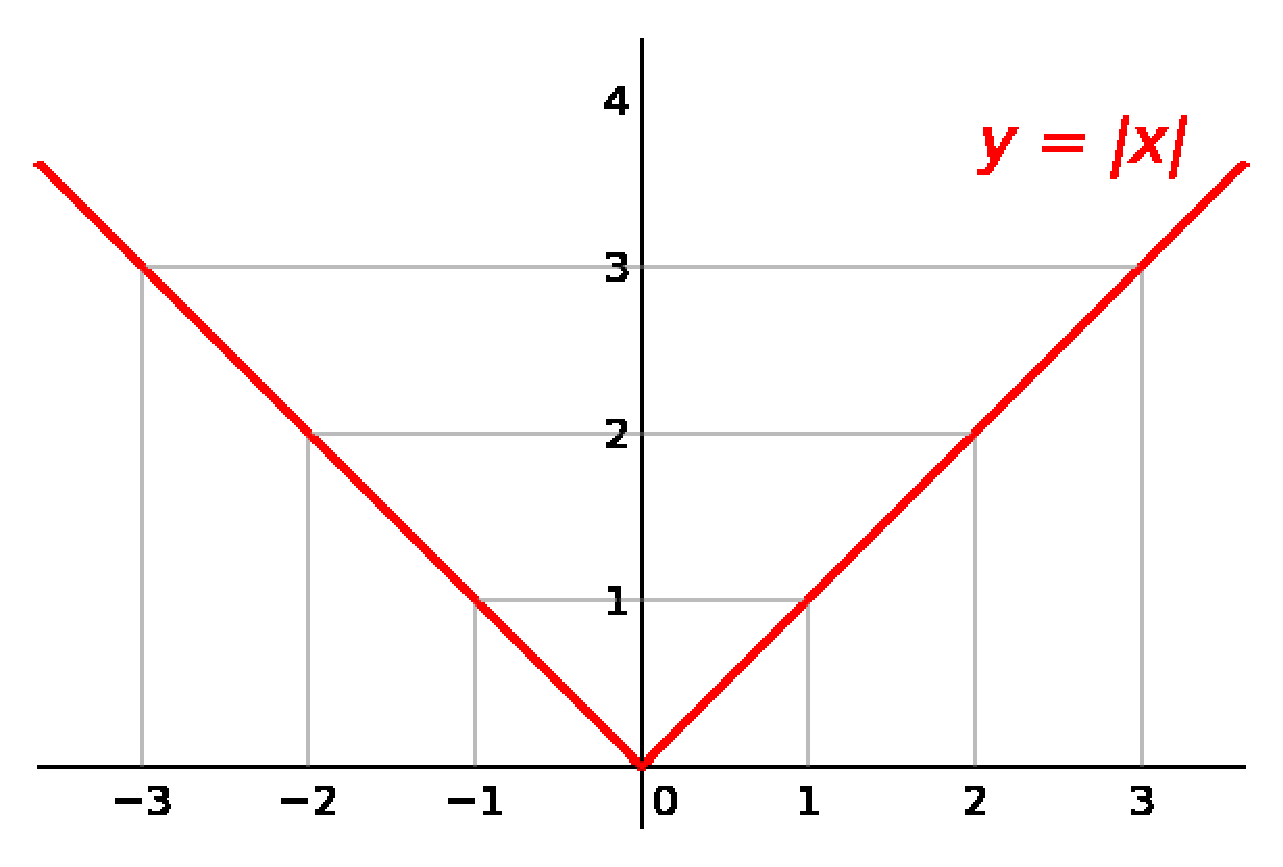
\includegraphics[height=5cm]{2_elem_rekenvaardigheden_B/inputs/Absolute_value_svg} 
%\end{figure}

We hebben er toen ook op gewezen dat je voorzichtig moet
zijn met formules van het type $\sqrt{x^{2}}$.

Passen we dit toe op een functie die horizontaal verschoven
is: $y=\sqrt{(x-1)^{2}}=\left|x-1\right|$.

Als deze functie zou gegeven zijn als de veelterm $x^{2}-2x+1$,
dan loont het dus de moeite om dit te herschrijven als een volledig
kwadraat: ${\displaystyle x^{2}-2x+1=\left(x-1\right)^{2}}$.


\subsubsection{De signum functie}

De sign of signum functie $\textrm{sgn}(x)$ is een eenvoudige wiskundige
functie, die eigenlijk het teken van het argument aangeeft:

\begin{equation*}
\textrm{sgn}(x)=\begin{cases}
-1 & \textrm{als}\:x<0\\
0 & \textrm{\textrm{als}}\:x=0\\
+1 & \textrm{\textrm{als}}\:x>0
\end{cases}
\end{equation*}

De grafiek van de signum functie:

\gewonefiguur{width=5cm}{2_elem_rekenvaardigheden_B/inputs/Signum_function_svg}
